\section{Motivation --- Cloud-centric Usage Management}

% Outline
% I. Frame the problem (use the AF proposal for this)
% II. Outline current solutions from UCDMO using guards
% III. Discuss problems (use pro/con list)
% IV. Frame specific challenges using slides II, III

\begin{frame}[t]
\frametitle{The Problem --- Customer Perspectives}
Current policy-centric systems are being forced to move to cloud environments and build much more open systems:
\newline
\newline
\newline
"...It is imperative to  effectively exchange information among components, Federal agencies, coalition partners, foreign governments and international organizations as a critical element of our efforts to defend the nation and execute national strategy..."\cite{proposal:info-sharing-strategy}
\newline
\begin{footnotesize}\textit{--- DoD Information Sharing Strategy}\end{footnotesize}
\newline
\newline
\newline
"...The CIO of the National Security Agency is focusing on IT architecture and a cloud-centric approach to sharing information..."\cite{proposal:nsa-cloud}
\newline
\begin{footnotesize}\textit{--- Informationweek}\end{footnotesize}
\end{frame}

\begin{frame}[t]
\frametitle{The Problem --- Characteristics}
Cloud systems may save money, provide more flexibility, but they also \cite{proposal:privacy-security-trust-cloud}:
\begin{itemize}
\item<2-> \textit{Are Not Private} --- User data control in SaaS is lacking, causing policy concerns for agencies; Data owners have no technical control over secondary use; providers may use offshore development; data can be routed across sensitive countries or secondarily stored on CDNs; data privacy on bankruptcy is ill-defined
\item<3-> \textit{Are Less Secure} --- Data owners no longer completely control data access, data may not be wiped in all XaaS scenarios, availability and backup leads to possible data proliferation, lack of standardization in intercloud communication and data transfer, multi-tenancy exposure to side-channel attacks, difficulty with reliable logging and auditing
\item<4-> \textit{Cannot Be Trusted} --- Trust relationships, consumer trust
\end{itemize}
\end{frame}

\begin{frame}[t]
\frametitle{Current Solutions}
How are these problems being addressed by impacted organizations?
\newline
\newline
\pause
They're just starting to be actively addressed and are an open research question \cite{proposal:assured-info-sharing}.
\newline
\newline
Cross-domain architectures are currently the standard for monitoring and information dissemination in an effort lead by the \textit{Unified Cross Domain Management Office}, associated with the Department of Defense (DoD) and the National Security Agency (NSA).
\end{frame}

\begin{frame}[t]
\frametitle{Current Solutions --- NSA}
Legacy cross-domain notional architecture \cite{proposal:nsa-arch}
\begin{figure}[!t]
\centering
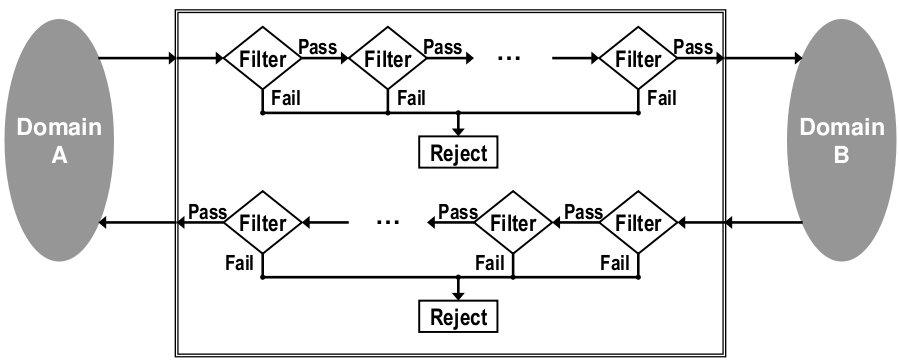
\includegraphics[width=3.4in]{nsa-legacy-arch}
\caption{NSA Legacy Model}
\label{fig:model:conceptual-model}
\end{figure}

\textit{Domain A} --- Private cloud managed by the Air Force
\newline
\textit{Domain B} --- A public operational network
\end{frame}

\begin{frame}[t]
\frametitle{Current Solutions --- NSA (SoA)}
Future cross-domain notional architecture \cite{proposal:nsa-arch}
\begin{figure}[!t]
\centering
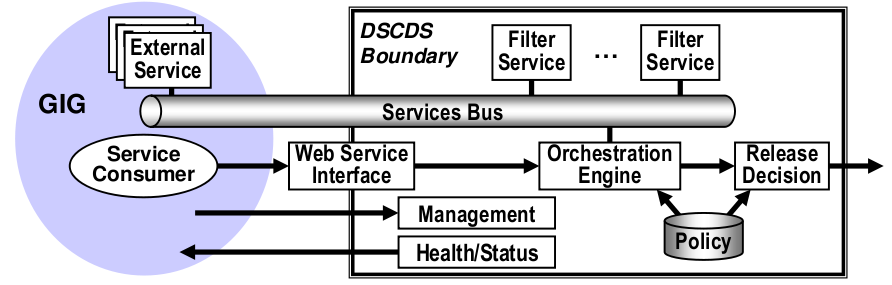
\includegraphics[width=3.4in]{nsa-arch}
\caption{NSA Service-Oriented Model}
\label{fig:model:conceptual-model}
\end{figure}

\textit{GiG} --- Global Information Grid; a large public cloud operated by the DoD
\newline
\textit{DSCDS} --- Distributed Service-oriented Cross Domain Solution
\end{frame}

\begin{frame}[t]
\frametitle{Current Solutions --- Raytheon}
Raytheon's notional architecture supporting cross-domain information flow \cite{proposal:raytheon-arch}:
\begin{figure}[!t]
\centering
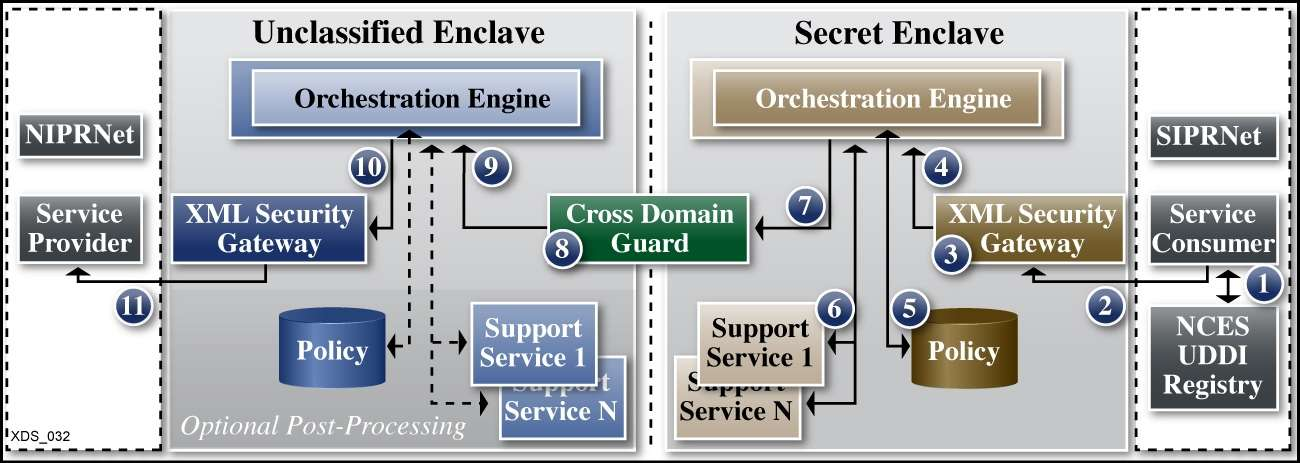
\includegraphics[width=3.4in]{raytheon-arch}
\caption{Raytheon Model}
\label{fig:model:conceptual-model}
\end{figure}

\textit{...still uses a single perimeter guard...}
\end{frame}

\begin{frame}[t]
\frametitle{Current Solutions --- BAH}
Booz|Allen|Hamilton presented a service-centric cross domain solution in 2009 \cite{proposal:bah-arch}:
\begin{figure}[!t]
\centering
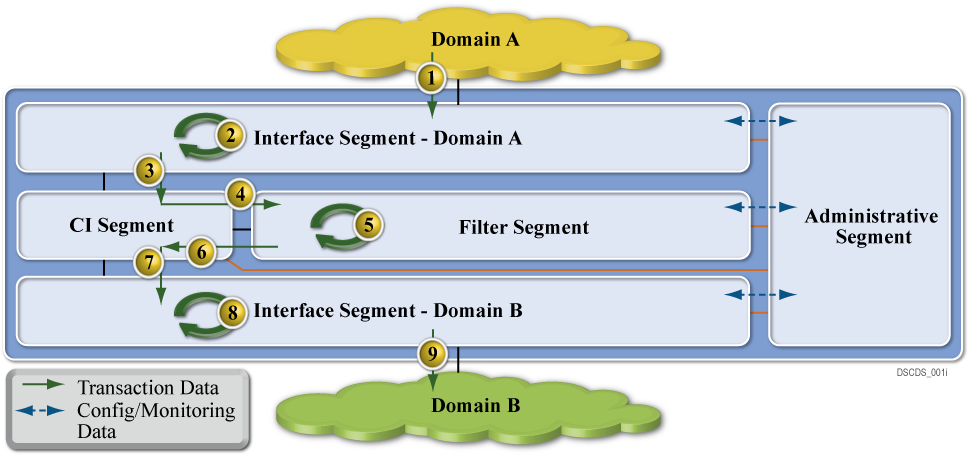
\includegraphics[width=3.4in]{bah-arch}
\caption{Booz|Allen|Hamilton Model}
\label{fig:model:conceptual-model}
\end{figure}
\textit{...still uses a single perimeter guard (called a filter segment)...}
\end{frame}

\begin{frame}[t]
\frametitle{Future Solution}
Organizations are falling back on what they know in the scope of new problems.
\begin{figure}[!t]
\centering
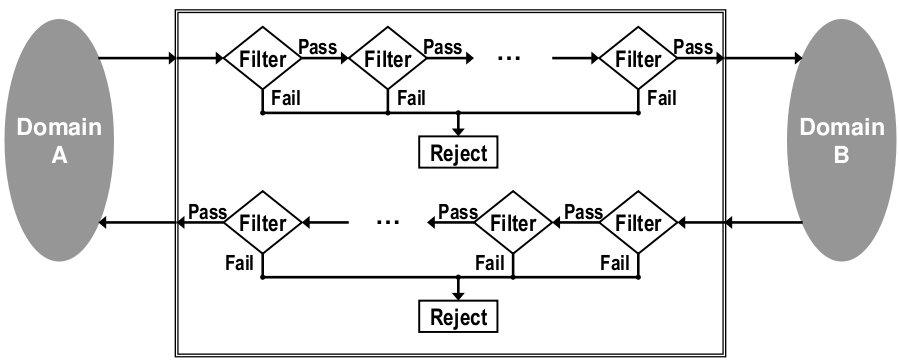
\includegraphics[width=3.4in]{nsa-legacy-arch}
\caption{NSA Legacy Model}
\label{fig:model:conceptual-model}
\end{figure}
\end{frame}

%overlay:
%- Policy into network fabric
%- Multiple compartments on same physical network
%- Network can integrate cloud components securely
%- Provides security in depth
%
%traditional/guard:
%- Policy centralized single points of failure
%- Each physical network can only be at one compartment level
%- Use is tied to the physical network; no cloud integration possible
%- Boundary security only 
\begin{frame}
\frametitle{Characteristics of Current Solutions}
\begin{itemize}
\item<2-> \textit{Centralized Policy} ---
\item<3-> \textit{Physical to Compartment Mapping} ---
\item<4-> \textit{Perimeter Protection} ---
\end{itemize}
\end{frame}
